\chapter{Specific requirements}

\section{External interface requirements}

The system provides all the main functions described in section 2.2.1.
Users are able to access all the information they are granted permission for.
Given such purposes, any device is suitable to make use of all the S\&C functionalities, allowing convenient access through any web browser.

\subsection{User Interfaces}

\begin{figure}[H]
    \centering
    \begin{minipage}{0.45\textwidth}
        \centering
        \fcolorbox{gray}{white}{
            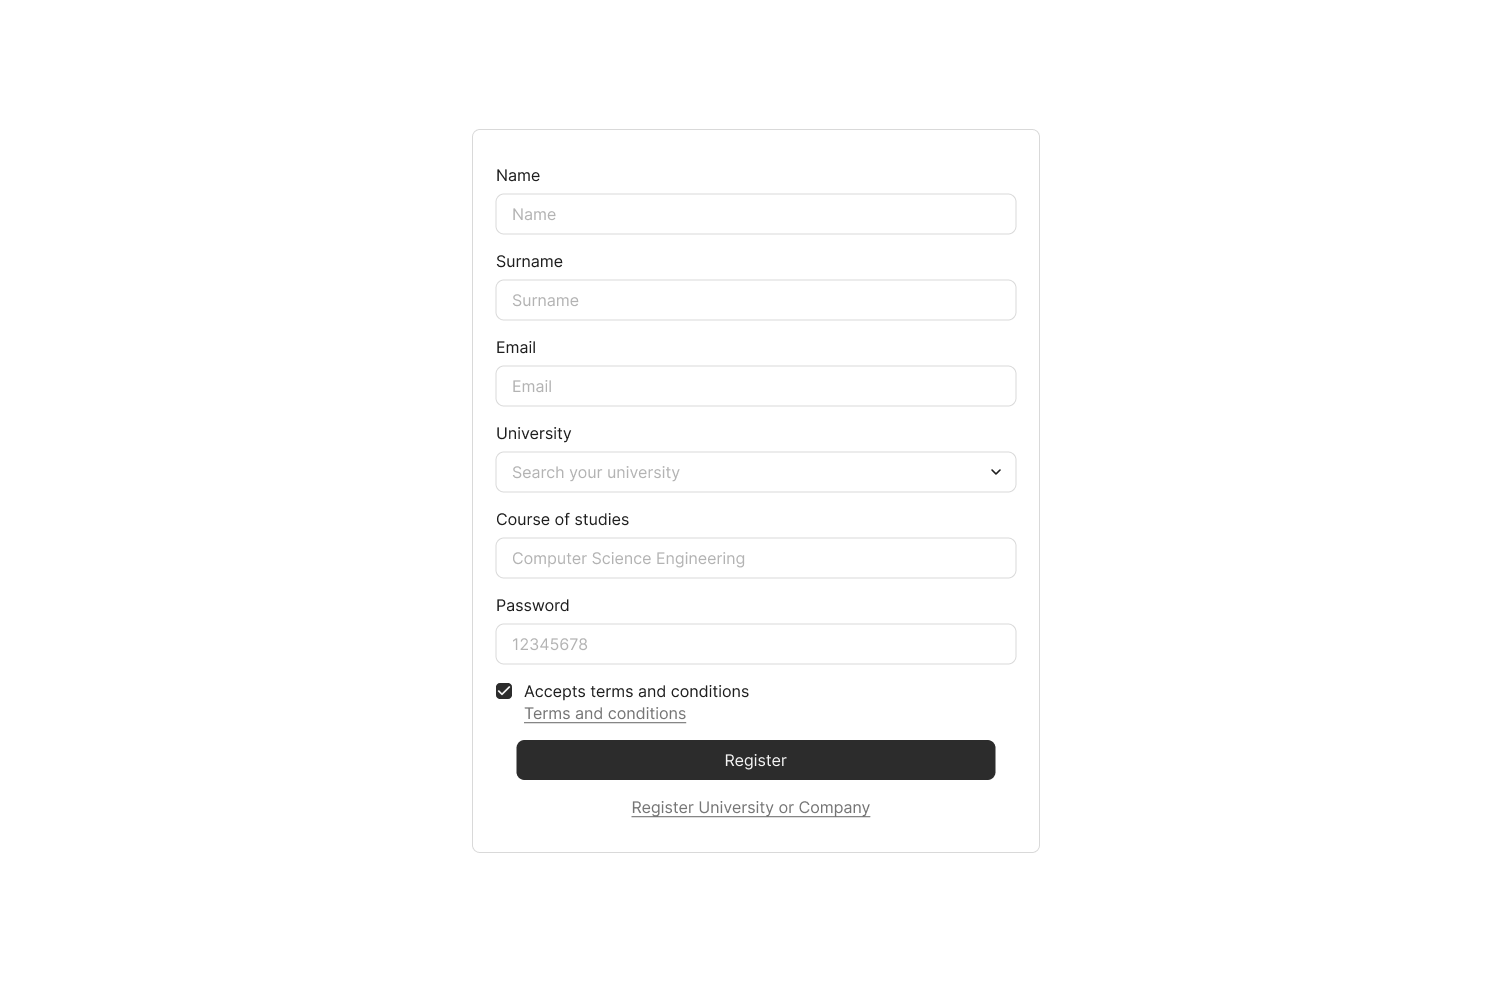
\includegraphics[width=\linewidth]{../../assets/user-interfaces/signup.png}
        }
        \subcaption{Sign up page}
    \end{minipage}
    \hfill
    \begin{minipage}{0.45\textwidth}
        \centering
        \fcolorbox{gray}{white}{
            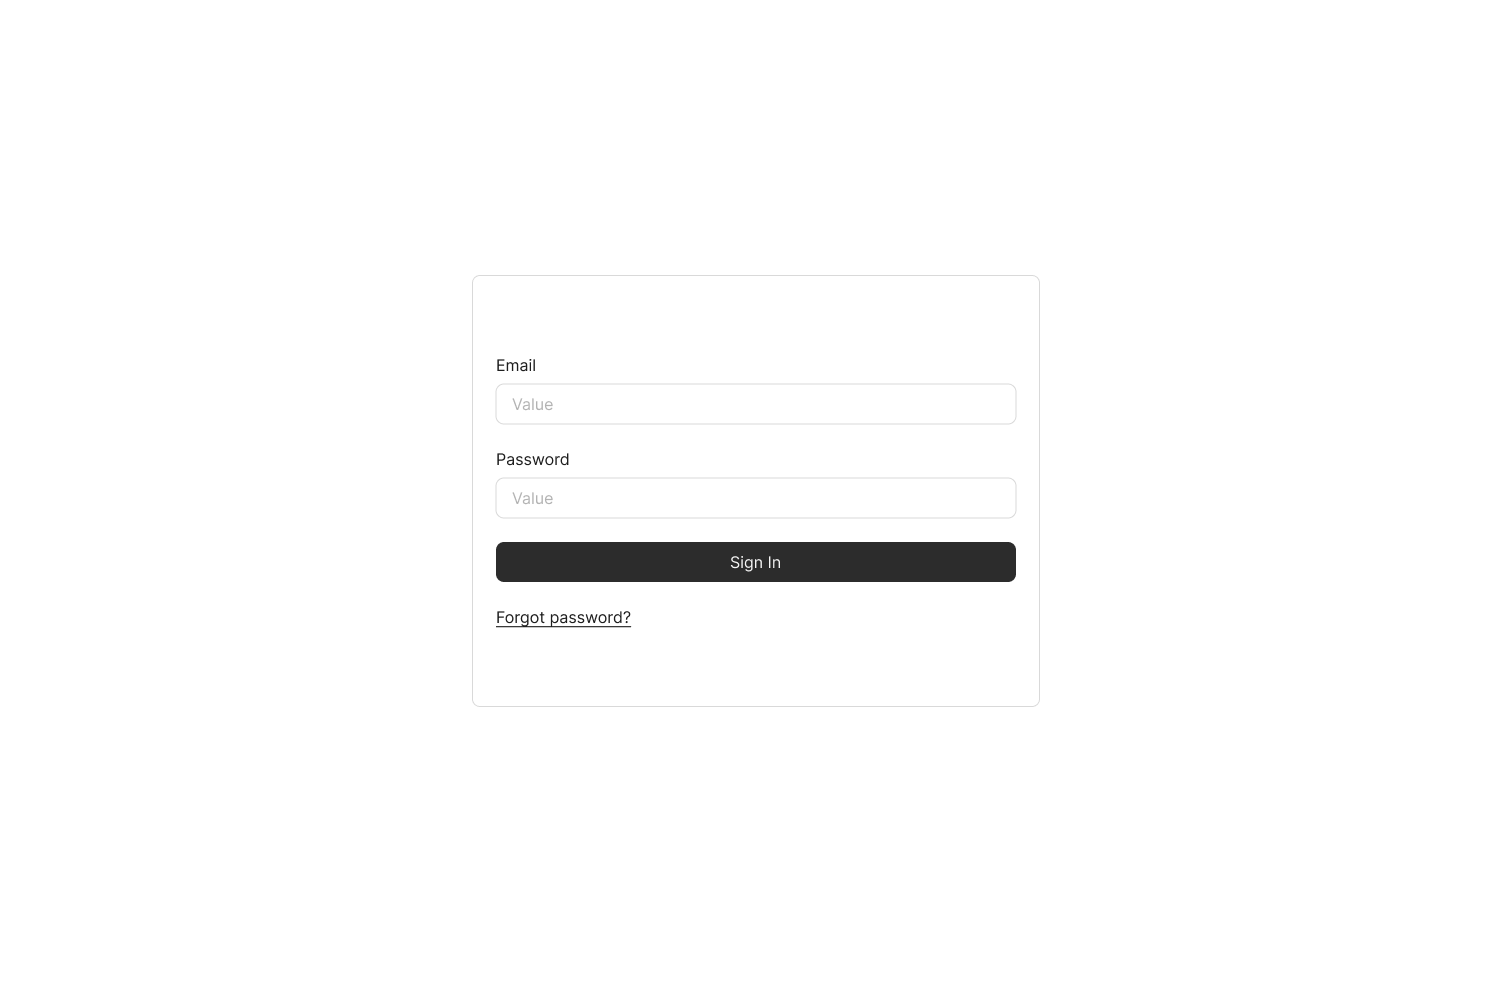
\includegraphics[width=\linewidth]{../../assets/user-interfaces/login.png}
        }
        \subcaption{Log in page}
    \end{minipage}

    \vspace{3em}

    \begin{minipage}{0.45\textwidth}
        \centering
        \fcolorbox{gray}{white}{
            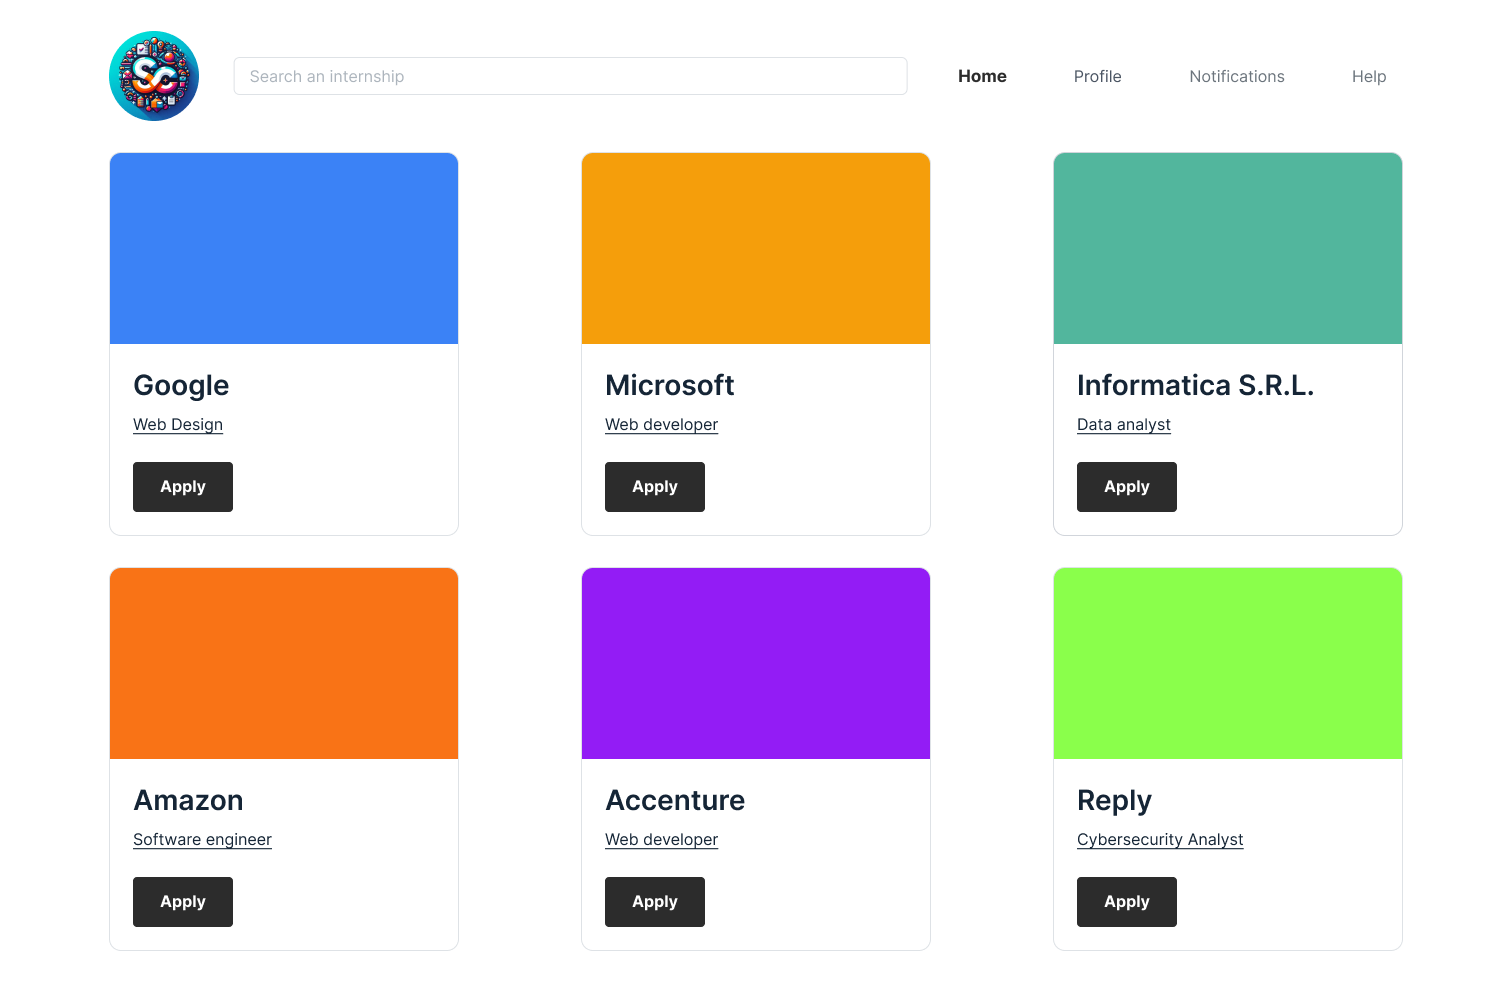
\includegraphics[width=\linewidth]{../../assets/user-interfaces/home.png}
        }
        \subcaption{Home page}
    \end{minipage}
    \hfill
    \begin{minipage}{0.45\textwidth}
        \centering
        \fcolorbox{gray}{white}{
            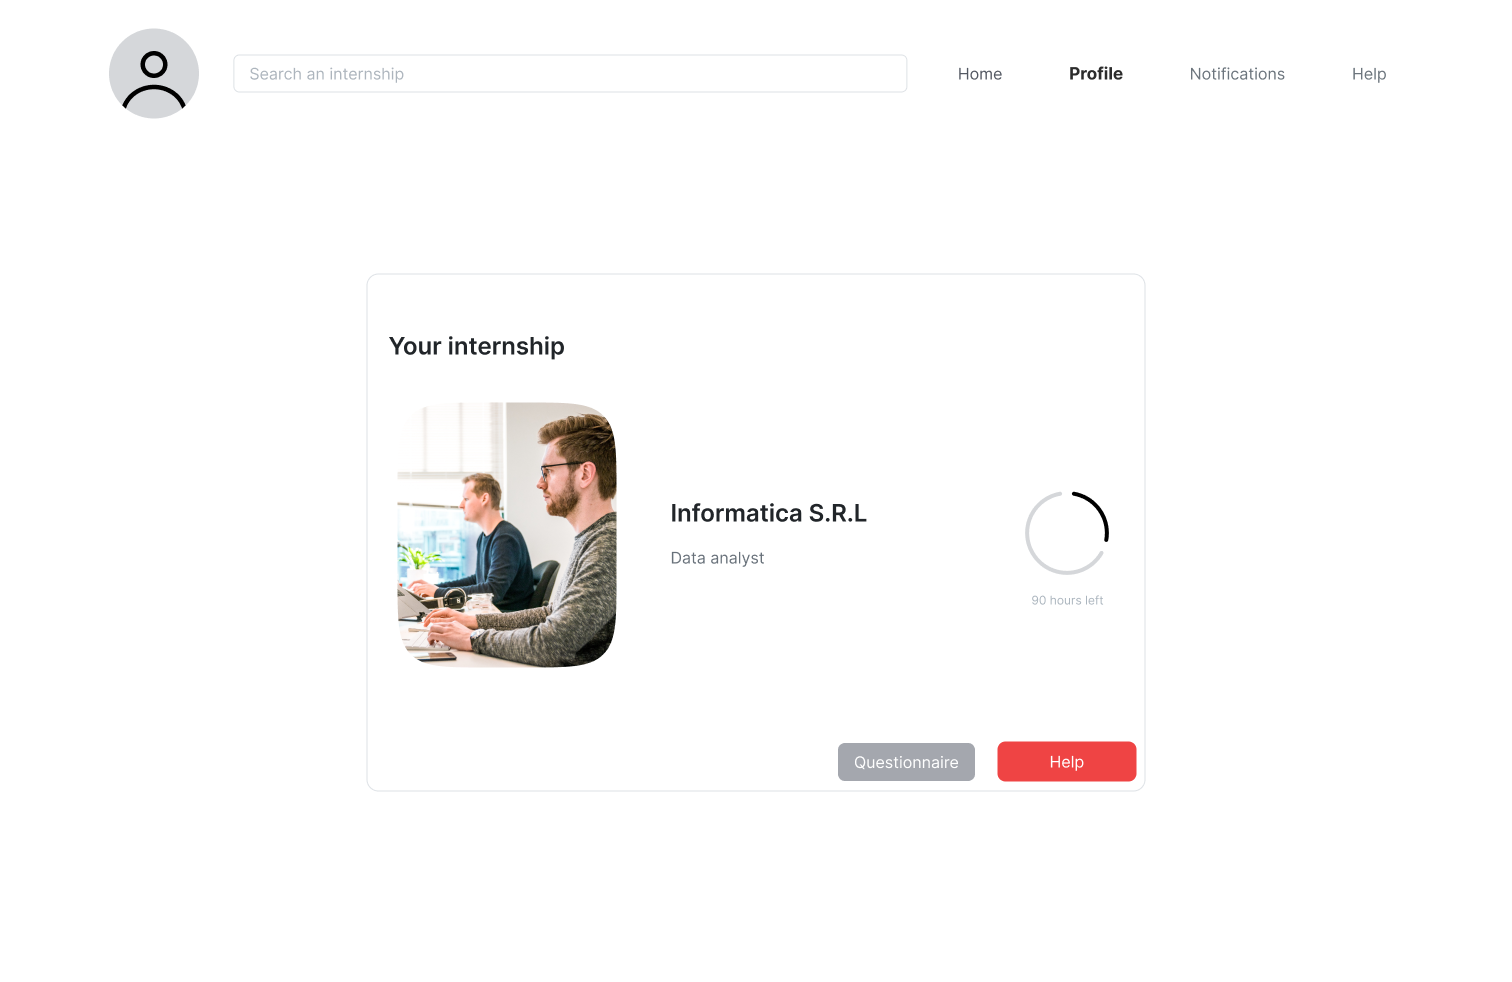
\includegraphics[width=\linewidth]{../../assets/user-interfaces/profile.png}
        }
        \subcaption{Profile page}
    \end{minipage}

    \vspace{3em}

    \begin{minipage}{0.45\textwidth}
        \centering
        \fcolorbox{gray}{white}{
            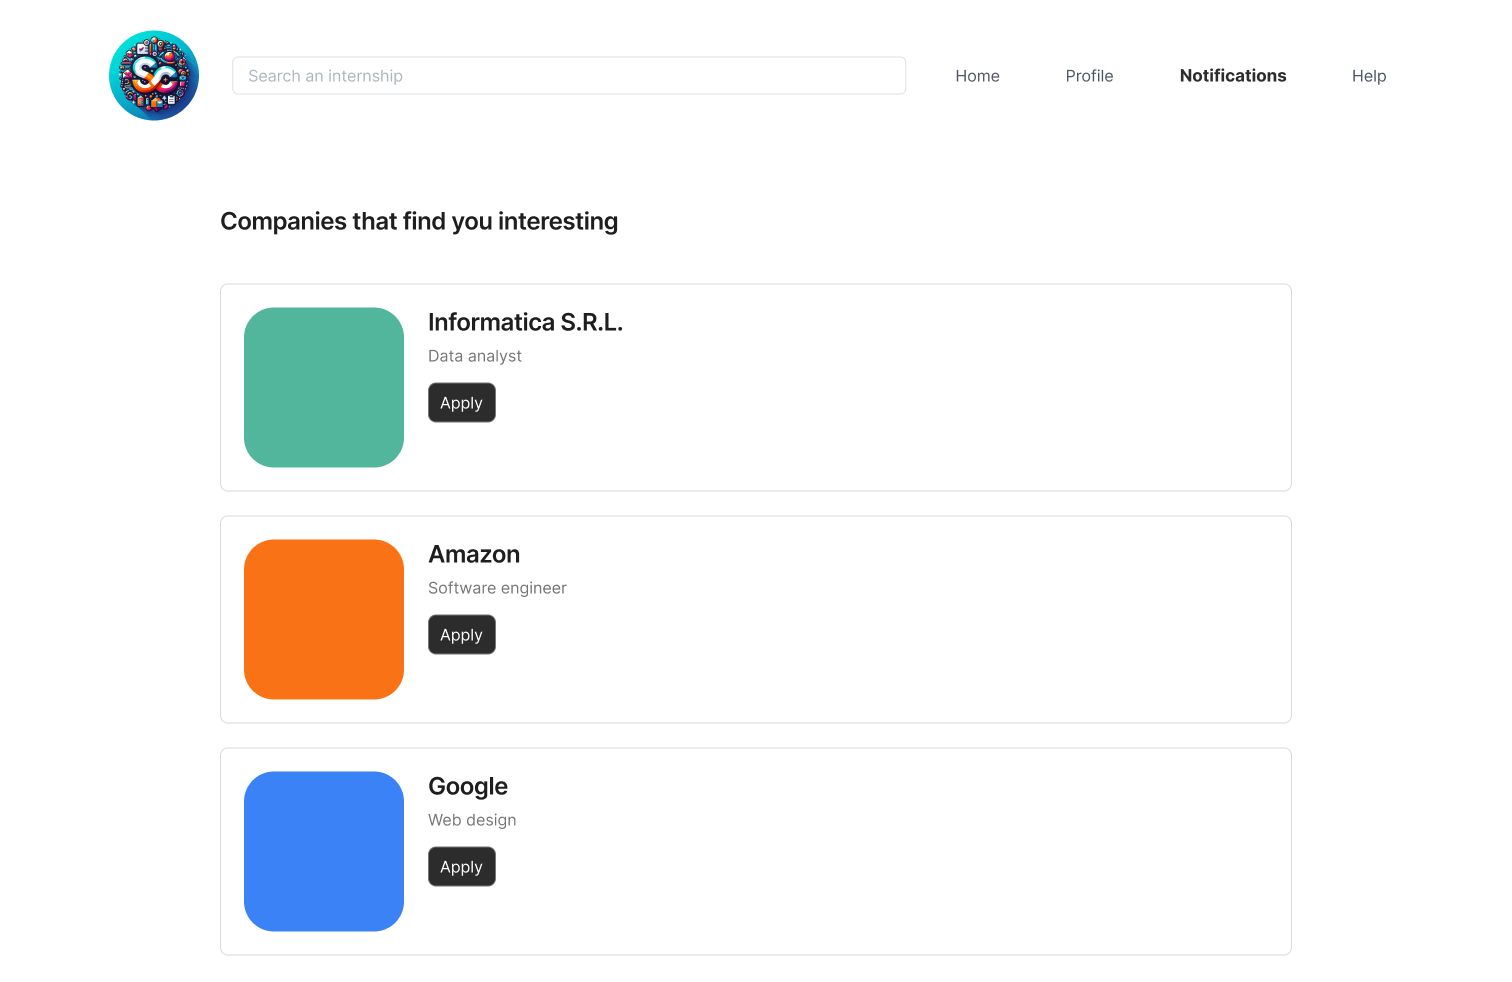
\includegraphics[width=\linewidth]{../../assets/user-interfaces/notifications.png}
        }
        \subcaption{Notifications page}
    \end{minipage}
    \hfill
    \begin{minipage}{0.45\textwidth}
        \centering
        \fcolorbox{gray}{white}{
            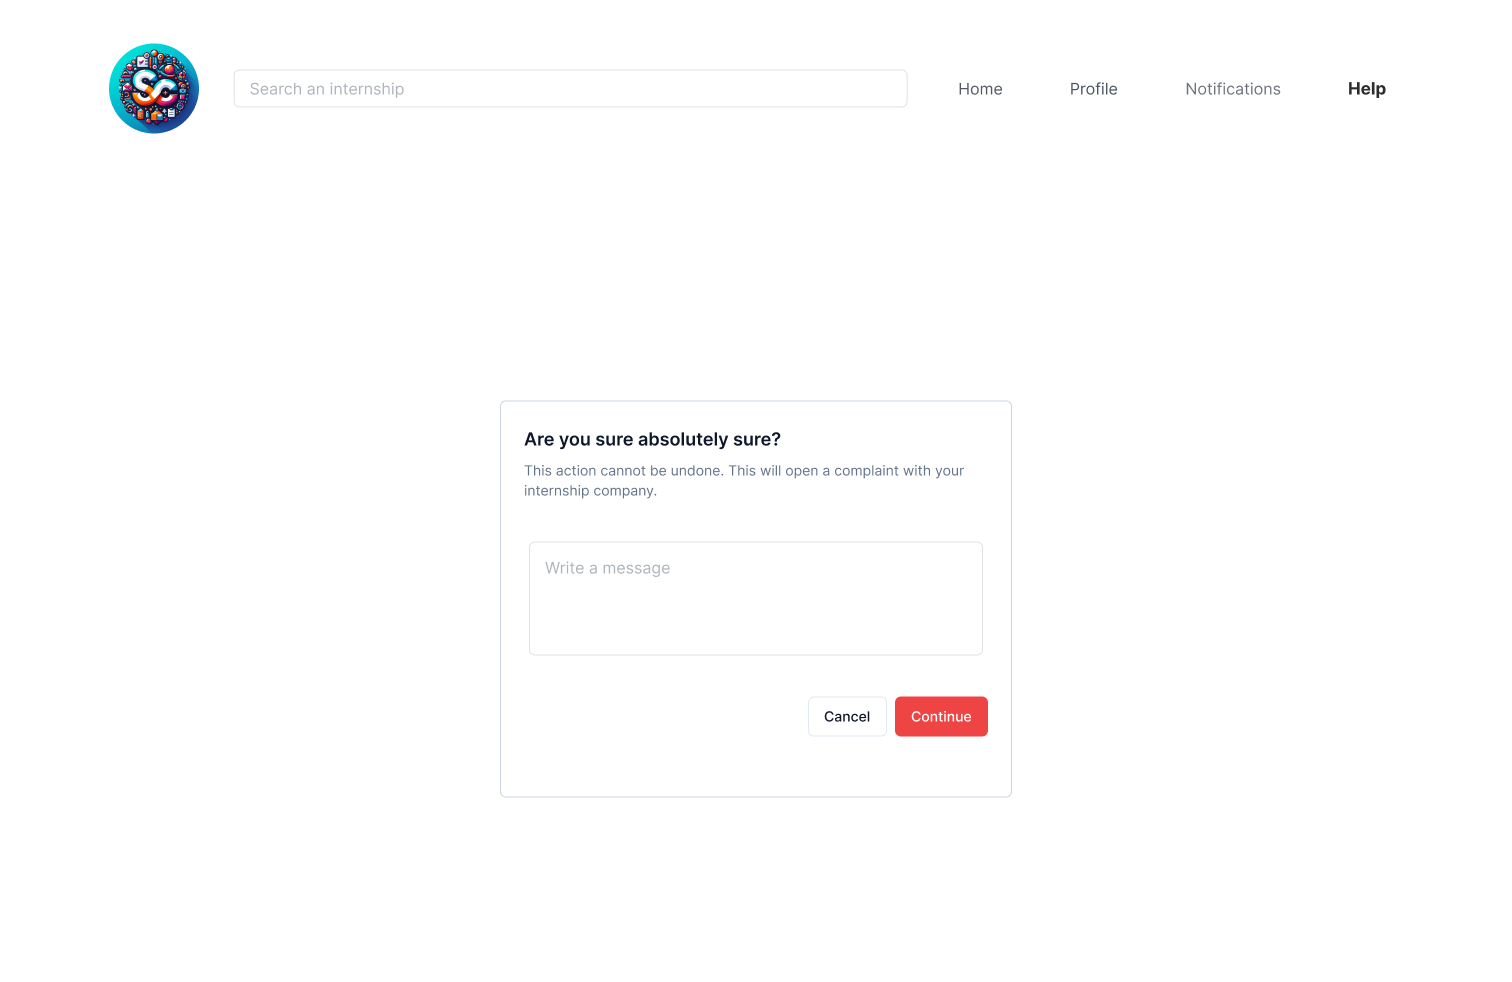
\includegraphics[width=\linewidth]{../../assets/user-interfaces/complaint.png}
        }
        \subcaption{Complaint page}
    \end{minipage}
\end{figure}

\subsection{Hardware Interfaces}

In order be accessed, the platform requires a suitable device with a web browser.

\subsection{Software Interfaces}

The system should integrate a notification service to keep users up of any event on the platform.
An email service is used for the registration process.

\subsection{Communication Interfaces}

The system requires a stable internet connection to work properly.
The connection is used to exchange data between users and the web server, which queries the requested information in a DB.

\section{Functional requirements}

\subsection{Use cases diagrams}

\begin{figure}[H]
    \centering
    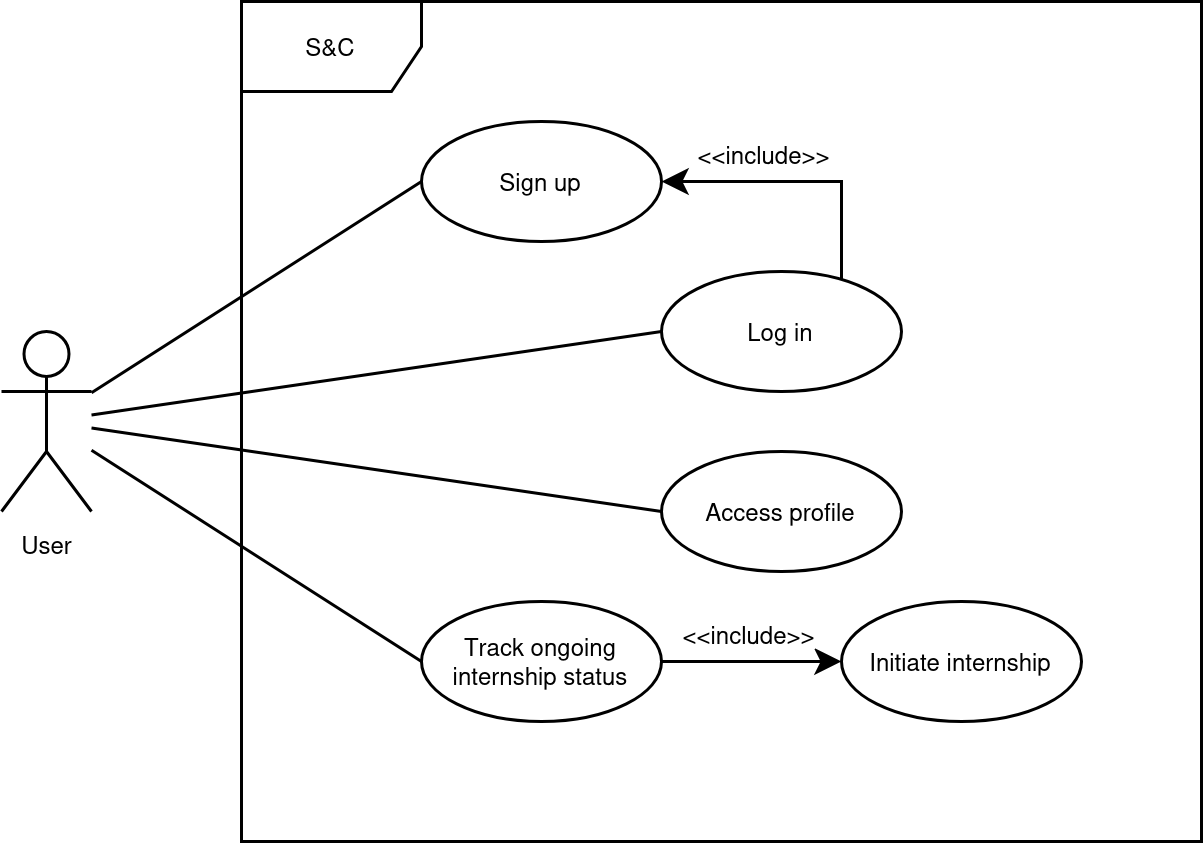
\includegraphics[width=0.3\linewidth]{../../assets/use-case-diagrams/user-common.png}
    \subcaption*{User common use cases}
\end{figure}

\begin{figure}[H]
    \centering
    \begin{minipage}{0.3\textwidth}
        \centering
        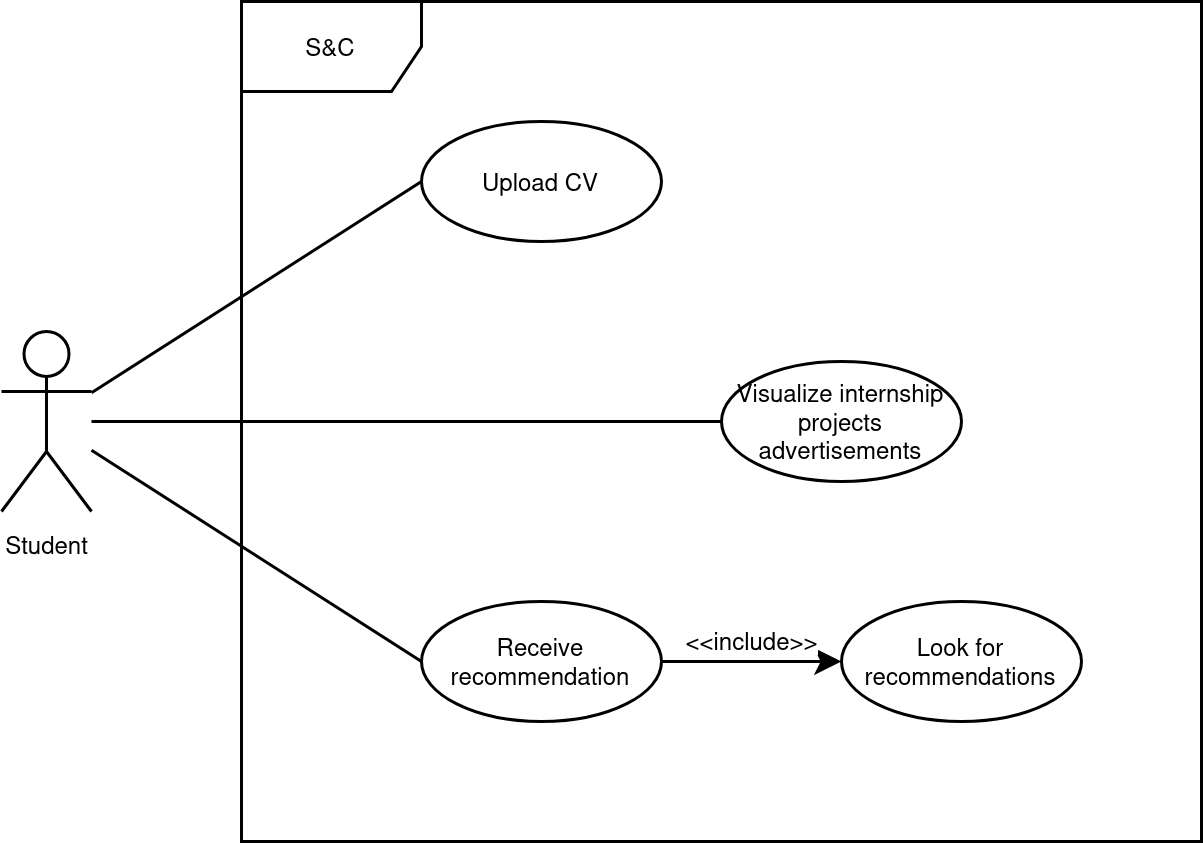
\includegraphics[width=\linewidth]{../../assets/use-case-diagrams/student-unique.png}
        \subcaption*{Student unique use cases}
    \end{minipage}
    \hspace{1in}
    \begin{minipage}{0.3\textwidth}
        \centering
        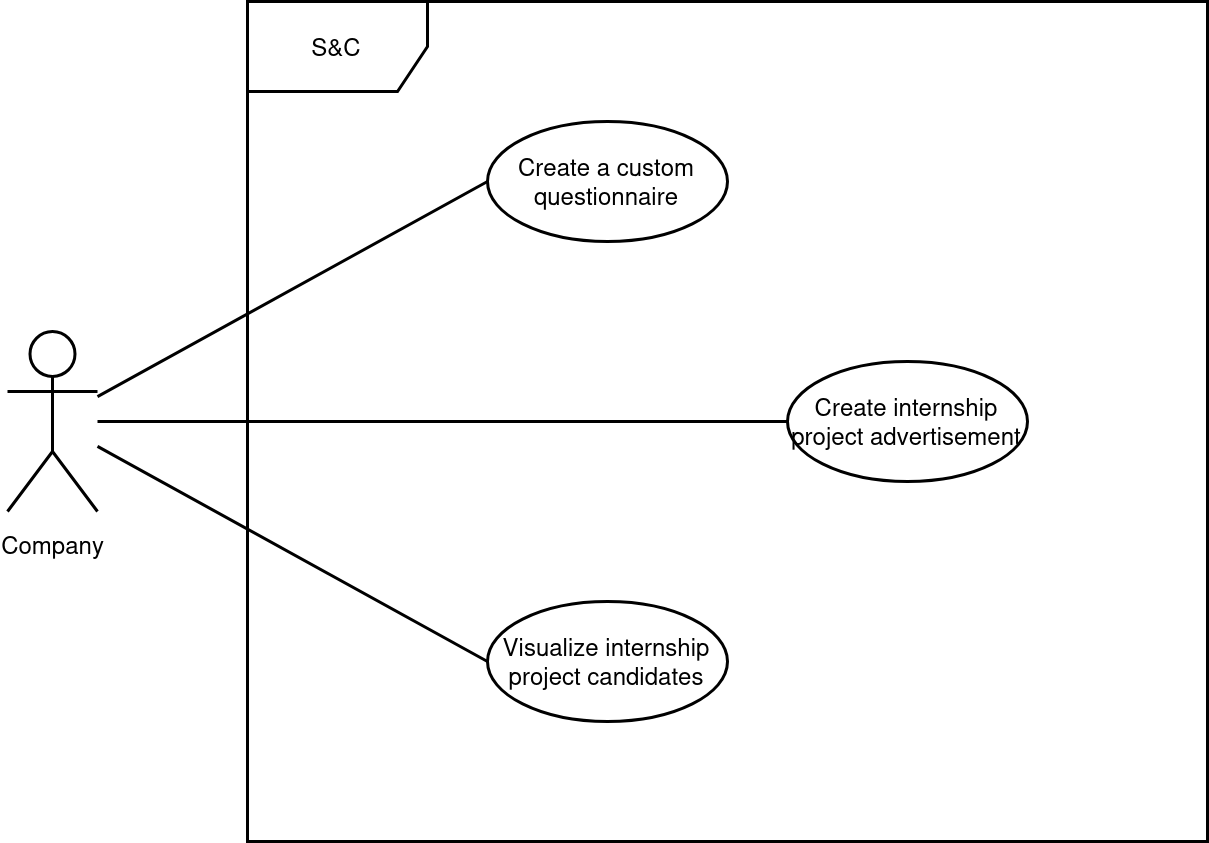
\includegraphics[width=\linewidth]{../../assets/use-case-diagrams/company-unique.png}
        \subcaption*{Company unique use cases}
    \end{minipage}
\end{figure}

\begin{figure}[H]
    \centering
    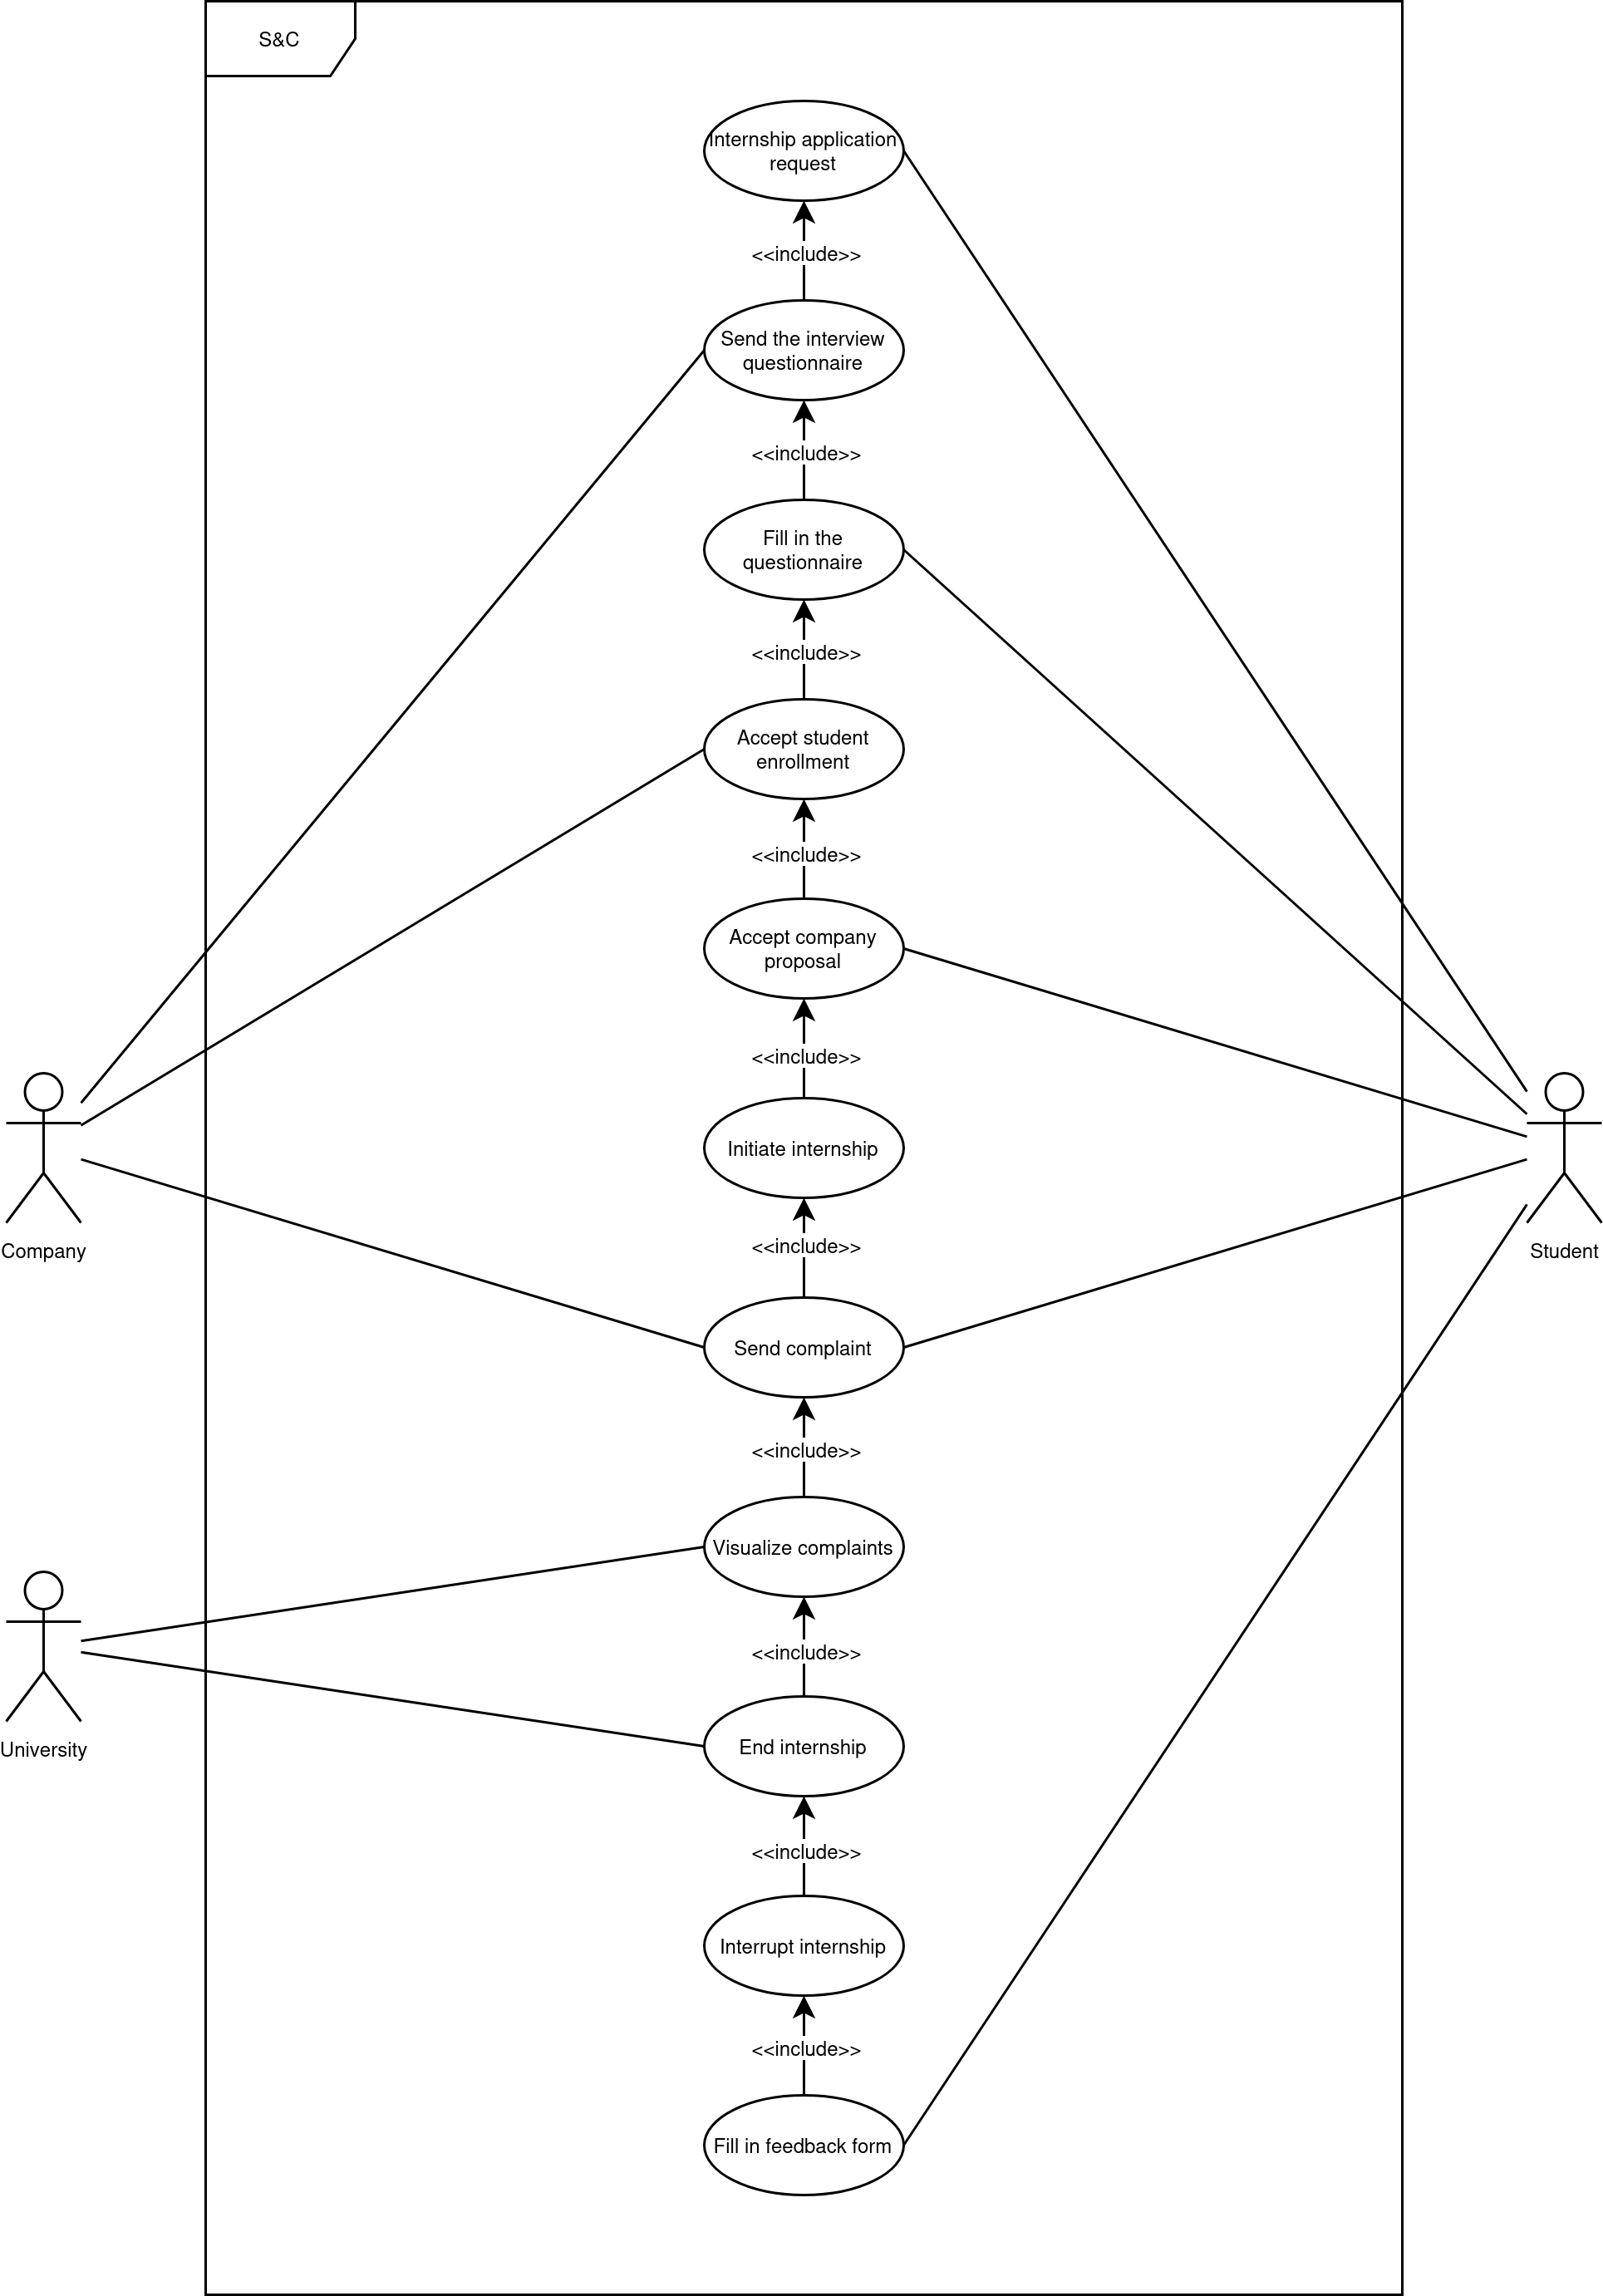
\includegraphics[width=0.8\linewidth]{../../assets/use-case-diagrams/internship-iter.png}
    \subcaption*{Internship iter use cases}
\end{figure}

\subsection{Use cases descriptions}

\begin{enumerate}[label=\textbf{UC\arabic* -}]

\item \subsubsection{StudentSignsUp}

\begin{table}[H]
    \centering
    \begin{tabular}{|l|m{10cm}|}
        \hline \multicolumn{2}{|c|}{\textbf{StudentSignsUp}} \\
        \hline \textbf{Actor} & Student, Students\&Companies, EmailService \\
        \hline \textbf{Entry condition} & The student is not already registered \\
        \hline \textbf{Event flow} &
            \begin{enumerate}[label=\arabic*]
                \item The student opens the sign up page
                \item The student fills in the required information and clicks the sign up button
                \item The platform checks that the information provided is valid
                \item The platform sends an email through the email service to verify the student account
                \item The student verifies the account via the link found in the email
                \item The platform registers the new student account
                \item The platform shows the student feed page
            \end{enumerate} \\
        \hline \textbf{Exit condition} & The student is registered \\
        \hline \textbf{Exceptions} & The student is already registered (3) \\
        \hline
    \end{tabular}
\end{table}

\item \subsubsection{CompanySignsUp}

\begin{table}[H]
    \centering
    \begin{tabular}{|l|m{10cm}|}
        \hline \multicolumn{2}{|c|}{\textbf{CompanySignsUp}} \\
        \hline \textbf{Actor} & Company, Students\&Companies, EmailService \\
        \hline \textbf{Entry condition} & The company is not already registered \\
        \hline \textbf{Event flow} &
            \begin{enumerate}[label=\arabic*]
                \item The company opens the sign up page
                \item The company fills in the required information and clicks the sign up button
                \item The platform checks that the information provided is valid
                \item The platform sends an email through the email service to verify the company account
                \item The company verifies the account via the link found in the email
                \item The platform registers the new company account
                \item The platform shows the company feed page
            \end{enumerate} \\
        \hline \textbf{Exit condition} & The company is registered \\
        \hline \textbf{Exceptions} & The company is already registered (3) \\
        \hline
    \end{tabular}
\end{table}

\item \subsubsection{UserLogsIn}

\begin{table}[H]
    \centering
    \begin{tabular}{|l|m{10cm}|}
        \hline \multicolumn{2}{|c|}{\textbf{UserLogsIn}} \\
        \hline \textbf{Actor} & Student, Company, University, Students\&Companies \\
        \hline \textbf{Entry condition} & User is registered \\
        \hline \textbf{Event flow} &
            \begin{enumerate}[label=\arabic*]
                \item The user opens the log in page
                \item The user enters its credentials and clicks the log in button
                \item The platform checks that the account exists and the credentials are correct
                \item The platform shows the home page
            \end{enumerate} \\
        \hline \textbf{Exit condition} & The user is logged in \\
        \hline \textbf{Exceptions} & The student is not registered (3) \\
        \hline
    \end{tabular}
\end{table}

\item \subsubsection{StudentUploadsCV}

\begin{table}[H]
    \centering
    \begin{tabular}{|l|m{10cm}|}
        \hline \multicolumn{2}{|c|}{\textbf{StudentUploadsCV}} \\
        \hline \textbf{Actor} & Student, Students\&Companies \\
        \hline \textbf{Entry condition} & The student is logged in \\
        \hline \textbf{Event flow} &
            \begin{enumerate}[label=\arabic*]
                \item The student opens the profile page
                \item The student clicks the upload CV button
                \item The student chooses the CV file and lets it upload
                \item The platform receives the file and stores it
                \item The platform shows the student profile page
            \end{enumerate} \\
        \hline \textbf{Exit condition} & The student profile page shows the new CV \\
        \hline \textbf{Exceptions} & None \\
        \hline
    \end{tabular}
\end{table}

\item \subsubsection{CompanyCreatesAdvertisement}

\begin{table}[H]
    \centering
    \begin{tabular}{|l|m{10cm}|}
        \hline \multicolumn{2}{|c|}{\textbf{CompanyCreatesAdvertisement}} \\
        \hline \textbf{Actor} & Company, Students\&Companies \\
        \hline \textbf{Entry condition} & The company is logged in \\
        \hline \textbf{Event flow} &
            \begin{enumerate}[label=\arabic*]
                \item The company opens the home page and clicks the create advertisement button
                \item The company writes out the advertisement details and clicks the post button
                \item The platform receives the advertisements details and stores it
                \item The platform shows the company home page
            \end{enumerate} \\
        \hline \textbf{Exit condition} & The advertisements can be found in the students feed \\
        \hline \textbf{Exceptions} & None \\
        \hline
    \end{tabular}
\end{table}

\item \subsubsection{StudentVisualizesAdvertisements}

\begin{table}[H]
    \centering
    \begin{tabular}{|l|m{10cm}|}
        \hline \multicolumn{2}{|c|}{\textbf{StudentVisualizesAdvertisements}} \\
        \hline \textbf{Actor} & Student, Students\&Companies \\
        \hline \textbf{Entry condition} & The student is logged in \\
        \hline \textbf{Event flow} &
            \begin{enumerate}[label=\arabic*]
                \item The student opens the feed page
                \item The platform searches suitable advertisements to show
                \item The platform sends the advertisements list to the student
                \item The student feed page shows the received list
            \end{enumerate} \\
        \hline \textbf{Exit condition} & The student visualizes interesting advertisements in the feed \\
        \hline \textbf{Exceptions} & None \\
        \hline
    \end{tabular}
\end{table}

\item \subsubsection{CompanyVisualizesCandidates}

\begin{table}[H]
    \centering
    \begin{tabular}{|l|m{10cm}|}
        \hline \multicolumn{2}{|c|}{\textbf{CompanyVisualizesCandidates}} \\
        \hline \textbf{Actor} & Company, Students\&Companies \\
        \hline \textbf{Entry condition} & The company is logged in \\
        \hline \textbf{Event flow} &
            \begin{enumerate}[label=\arabic*]
                \item The company opens the feed page
                \item The platform searches suitable students to show
                \item The platform sends the students list to the company
                \item The company feed page shows the received list
            \end{enumerate} \\
        \hline \textbf{Exit condition} & The company visualizes potential students in the feed \\
        \hline \textbf{Exceptions} & None \\
        \hline
    \end{tabular}
\end{table}

\item \subsubsection{CompanyCreatesQuestionnaire}

\begin{table}[H]
    \centering
    \begin{tabular}{|l|m{10cm}|}
        \hline \multicolumn{2}{|c|}{\textbf{CompanyCreatesQuestionnaire}} \\
        \hline \textbf{Actor} & Company, Students\&Companies \\
        \hline \textbf{Entry condition} & The company is logged in \\
        \hline \textbf{Event flow} &
            \begin{enumerate}[label=\arabic*]
                \item The company opens the home page and clicks the create questionnaire button
                \item The company builds the questionnaire form and clicks the save button
                \item The platform receives the questionnaire form and stores it
                \item The platform shows the company home page
            \end{enumerate} \\
        \hline \textbf{Exit condition} & The questionnaire can be sent to students who have applied \\
        \hline \textbf{Exceptions} & None \\
        \hline
    \end{tabular}
\end{table}

\item \subsubsection{StudentFillsQuestionnaire}

\begin{table}[H]
    \centering
    \begin{tabular}{|l|m{10cm}|}
        \hline \multicolumn{2}{|c|}{\textbf{StudentFillsQuestionnaire}} \\
        \hline \textbf{Actor} & Student, Students\&Companies \\
        \hline \textbf{Entry condition} & The student has received a questionnaire to fill \\
        \hline \textbf{Event flow} &
            \begin{enumerate}[label=\arabic*]
                \item The student opens the notifications page
                \item The student opens the questionnaire that the company has sent
                \item The student fills the questionnaire form and clicks the submit button
                \item The platform sends the filled questionnaire to the company
            \end{enumerate} \\
        \hline \textbf{Exit condition} & The company receives the filled questionnaire \\
        \hline \textbf{Exceptions} & None \\
        \hline
    \end{tabular}
\end{table}

\item \subsubsection{CompanyAcceptsStudentEnrollment}

\begin{table}[H]
    \centering
    \begin{tabular}{|l|m{10cm}|}
        \hline \multicolumn{2}{|c|}{\textbf{CompanyAcceptsStudentEnrollment}} \\
        \hline \textbf{Actor} & Student, Company, Students\&Companies \\
        \hline \textbf{Entry condition} & The student has sent the questionnaire back to the company \\
        \hline \textbf{Event flow} &
            \begin{enumerate}[label=\arabic*]
                \item The company opens the page with the student questionnaire
                \item The company reviews the questionnaire and clicks the accept student button
                \item The platform notifies the student that it has been accepted
                \item The student opens the notifications page and clicks the accept button
                \item The platform checks that all information is valid
                \item The platform initiates the internship between student and company
                \item The platform shows the internship page to the student
                \item The platform notifies the company that the internship has started
            \end{enumerate} \\
        \hline \textbf{Exit condition} & An internship is started between student and company \\
        \hline \textbf{Exceptions} & The student meanwhile accepted another internship (5) \\
        \hline
    \end{tabular}
\end{table}

\item \subsubsection{StudentVisualizesInternshipInformation}

\begin{table}[H]
    \centering
    \begin{tabular}{|l|m{10cm}|}
        \hline \multicolumn{2}{|c|}{\textbf{StudentVisualizesInternshipInformation}} \\
        \hline \textbf{Actor} & Student, Students\&Companies \\
        \hline \textbf{Entry condition} & Student is enrolled in an internship \\
        \hline \textbf{Event flow} &
            \begin{enumerate}[label=\arabic*]
                \item The student opens the profile page
                \item The student selects its internship project panel
                \item The platform shows the student internship information
            \end{enumerate} \\
        \hline \textbf{Exit condition} & The student visualizes its ongoing internship information \\
        \hline \textbf{Exceptions} & None \\
        \hline
    \end{tabular}
\end{table}

\item \subsubsection{CompanyVisualizesInternshipsInformation}

\begin{table}[H]
    \centering
    \begin{tabular}{|l|m{10cm}|}
        \hline \multicolumn{2}{|c|}{\textbf{CompanyVisualizesInternshipsInformation}} \\
        \hline \textbf{Actor} & Company, Students\&Companies \\
        \hline \textbf{Entry condition} & Company has students enrolled in its internships \\
        \hline \textbf{Event flow} &
            \begin{enumerate}[label=\arabic*]
                \item The company opens the profile page
                \item The company selects one of its active internship projects
                \item The platform shows the enrolled students and the internship information
            \end{enumerate} \\
        \hline \textbf{Exit condition} & The company visualizes its ongoing internship information \\
        \hline \textbf{Exceptions} & None \\
        \hline
    \end{tabular}
\end{table}

\item \subsubsection{StudentSendsComplaint}

\begin{table}[H]
    \centering
    \begin{tabular}{|l|m{10cm}|}
        \hline \multicolumn{2}{|c|}{\textbf{StudentSendsComplaint}} \\
        \hline \textbf{Actor} & Student, University, Students\&Companies \\
        \hline \textbf{Entry condition} & The student is currently enrolled in an internship \\
        \hline \textbf{Event flow} &
            \begin{enumerate}[label=\arabic*]
                \item The student opens the complaints page
                \item The student fills in the complaint text box and clicks the send button
                \item The platform notifies the university of the complaint
            \end{enumerate} \\
        \hline \textbf{Exit condition} & The university is notified of the complaint \\
        \hline \textbf{Exceptions} & None \\
        \hline
    \end{tabular}
\end{table}

\item \subsubsection{CompanySendsComplaint}

\begin{table}[H]
    \centering
    \begin{tabular}{|l|m{10cm}|}
        \hline \multicolumn{2}{|c|}{\textbf{CompanySendsComplaint}} \\
        \hline \textbf{Actor} & Company, University, Students\&Companies \\
        \hline \textbf{Entry condition} & The company has a student currently enrolled in its internship \\
        \hline \textbf{Event flow} &
            \begin{enumerate}[label=\arabic*]
                \item The company opens the complaints page
                \item The company fills in the complaint text box and clicks the send button
                \item The platform notifies the university of the complaint
            \end{enumerate} \\
        \hline \textbf{Exit condition} & The university is notified of the complaint \\
        \hline \textbf{Exceptions} & None \\
        \hline
    \end{tabular}
\end{table}

\item \subsubsection{UniversityVisualizesComplaints}

\begin{table}[H]
    \centering
    \begin{tabular}{|l|m{10cm}|}
        \hline \multicolumn{2}{|c|}{\textbf{UniversityVisualizesComplaints}} \\
        \hline \textbf{Actor} & University, Students\&Companies \\
        \hline \textbf{Entry condition} & A complaint has been sent by a student or a company \\
        \hline \textbf{Event flow} &
            \begin{enumerate}[label=\arabic*]
                \item The university opens the notifications/complaint page
                \item The university selects one complaint notification
                \item The university visualizes the full complaint message and information
            \end{enumerate} \\
        \hline \textbf{Exit condition} & The university visualizes the complaint \\
        \hline \textbf{Exceptions} & None \\
        \hline
    \end{tabular}
\end{table}

\item \subsubsection{UniversityEndsInternship}

\begin{table}[H]
    \centering
    \begin{tabular}{|l|m{10cm}|}
        \hline \multicolumn{2}{|c|}{\textbf{UniversityEndsInternship}} \\
        \hline \textbf{Actor} & Student, Company, University, Students\&Companies \\
        \hline \textbf{Entry condition} & Student and company are currently linked in an internship \\
        \hline \textbf{Event flow} &
            \begin{enumerate}[label=\arabic*]
                \item The university opens the ongoing internships page and clicks the interruption button
                \item The platform registers the internship as concluded
                \item The company is notified of the internship conclusion
                \item The student is notified of the internship conclusion
            \end{enumerate} \\
        \hline \textbf{Exit condition} & The internship is registered as concluded \\
        \hline \textbf{Exceptions} & None \\
        \hline
    \end{tabular}
\end{table}

\item \subsubsection{InternshipExpires}

\begin{table}[H]
    \centering
    \begin{tabular}{|l|m{10cm}|}
        \hline \multicolumn{2}{|c|}{\textbf{InternshipExpires}} \\
        \hline \textbf{Actor} & Student, Company, Students\&Companies \\
        \hline \textbf{Entry condition} & An ongoing internship reaches its conclusion date \\
        \hline \textbf{Event flow} &
            \begin{enumerate}[label=\arabic*]
                \item The platform sees that the internship has reached its conclusion date
                \item The platform registers the internship as concluded
                \item The company is notified of the internship conclusion
                \item The student is notified of the internship conclusion
            \end{enumerate} \\
        \hline \textbf{Exit condition} & The internship is registered as concluded \\
        \hline \textbf{Exceptions} & None \\
        \hline
    \end{tabular}
\end{table}

\item \subsubsection{StudentFillsFeedbackForm}

\begin{table}[H]
    \centering
    \begin{tabular}{|l|m{10cm}|}
        \hline \multicolumn{2}{|c|}{\textbf{StudentFillsFeedbackForm}} \\
        \hline \textbf{Actor} & Student, Students\&Companies \\
        \hline \textbf{Entry condition} & The internship has ended \\
        \hline \textbf{Event flow} &
            \begin{enumerate}[label=\arabic*]
                \item The platform notifies the student that a feedback form can be filled in
                \item The student opens the notifications page
                \item The student opens the feedback form page
                \item The student fills in the form and submits it
                \item The platform receives the feedback form and stores it
            \end{enumerate} \\
        \hline \textbf{Exit condition} & The platform receives feedback data about a company \\
        \hline \textbf{Exceptions} & None \\
        \hline
    \end{tabular}
\end{table}

\end{enumerate}

\subsection{Use cases sequence diagrams}

\begin{enumerate}[label=\textbf{UC\arabic* -}]

\item \subsubsection{StudentSignsUp}

\begin{figure}[H]
    \centering
    \fcolorbox{black}{white}{
        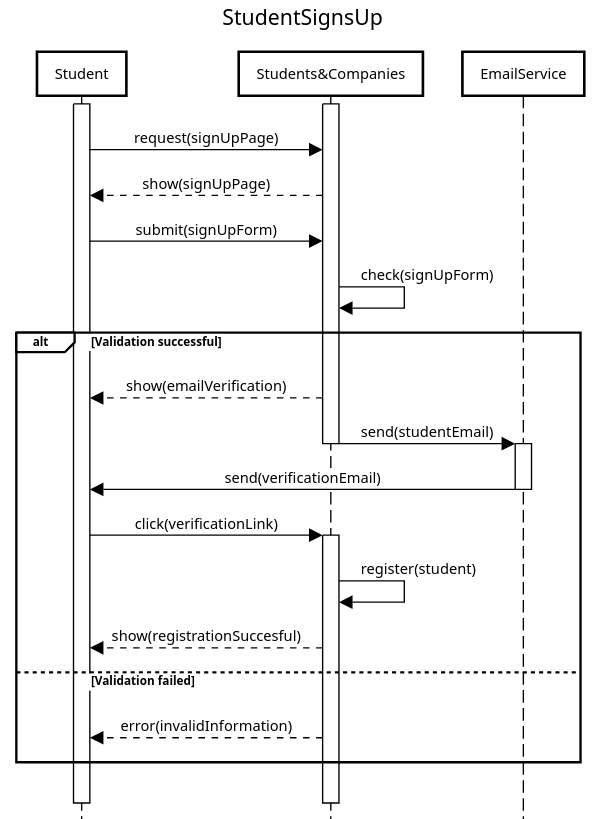
\includegraphics[width=0.8\textwidth]{../../assets/sequence-diagrams/StudentSignsUp.png}
    }
\end{figure}

\item \subsubsection{CompanySignsUp}

\begin{figure}[H]
    \centering
    \fcolorbox{black}{white}{
        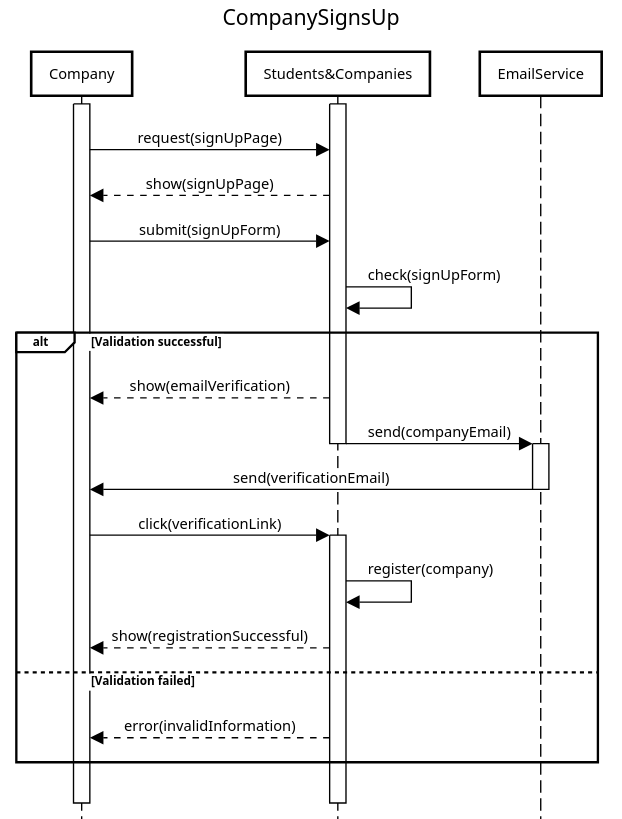
\includegraphics[width=0.8\textwidth]{../../assets/sequence-diagrams/CompanySignsUp.png}
    }
\end{figure}

\item \subsubsection{UserLogsIn}

\begin{figure}[H]
    \centering
    \fcolorbox{black}{white}{
        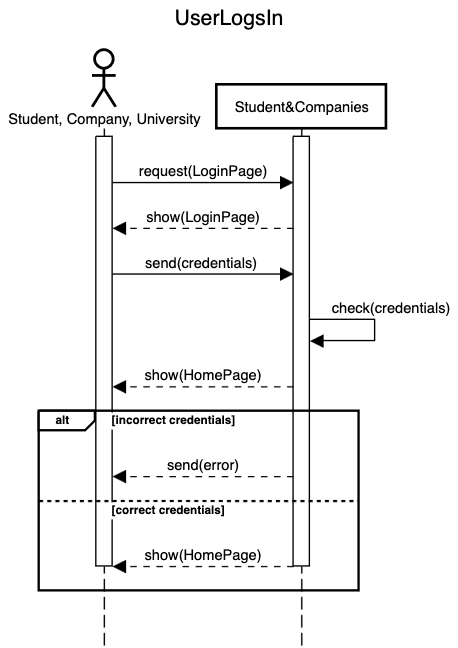
\includegraphics[width=0.5\textwidth]{../../assets/sequence-diagrams/UserLogsIn.png}
    }
\end{figure}

\item \subsubsection{StudentUploadsCV}

\begin{figure}[H]
    \centering
    \fcolorbox{black}{white}{
        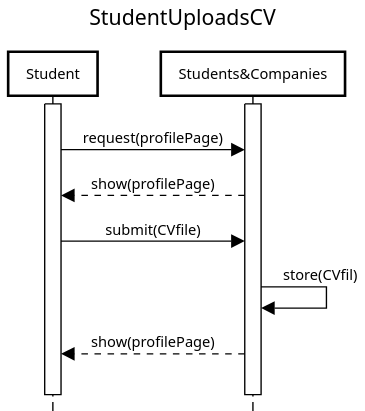
\includegraphics[width=0.5\textwidth]{../../assets/sequence-diagrams/StudentUploadsCV.png}
    }
\end{figure}

\item \subsubsection{CompanyCreatesAdvertisement}

\begin{figure}[H]
    \centering
    \fcolorbox{black}{white}{
        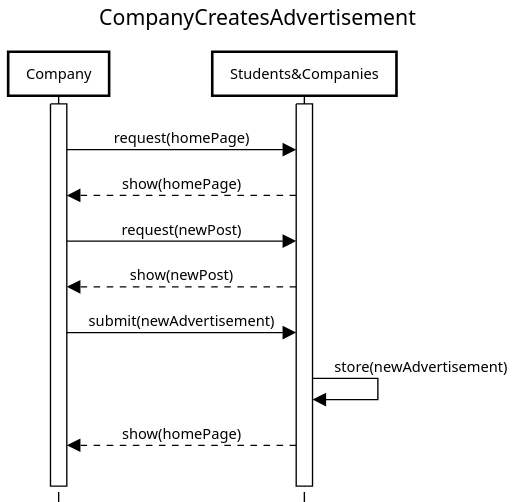
\includegraphics[width=0.5\textwidth]{../../assets/sequence-diagrams/CompanyCreatesAdvertisement.png}
    }
\end{figure}

\item \subsubsection{StudentVisualizesAdvertisements}

\begin{figure}[H]
    \centering
    \fcolorbox{black}{white}{
        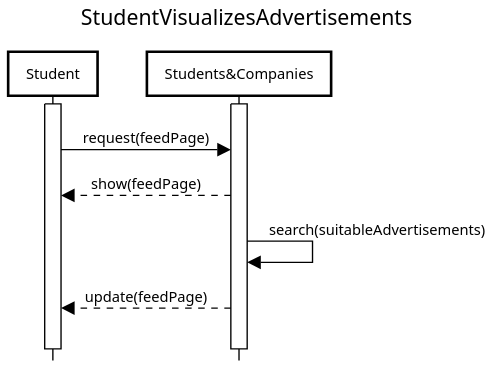
\includegraphics[width=0.5\textwidth]{../../assets/sequence-diagrams/StudentVisualizesAdvertisements.png}
    }
\end{figure}

\item \subsubsection{CompanyVisualizesCandidates}

\begin{figure}[H]
    \centering
    \fcolorbox{black}{white}{
        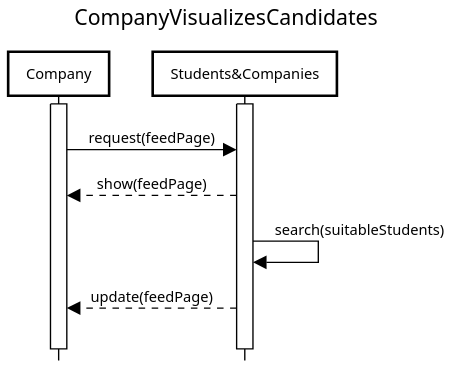
\includegraphics[width=0.5\textwidth]{../../assets/sequence-diagrams/CompanyVisualizesCandidates.png}
    }
\end{figure}

\item \subsubsection{CompanyCreatesQuestionnaire}

\begin{figure}[H]
    \centering
    \fcolorbox{black}{white}{
        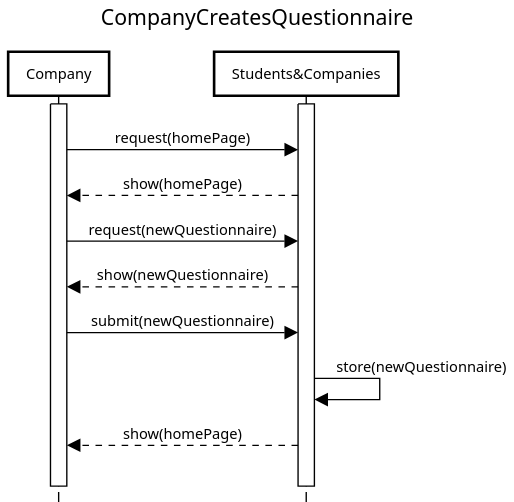
\includegraphics[width=0.5\textwidth]{../../assets/sequence-diagrams/CompanyCreatesQuestionnaire.png}
    }
\end{figure}

\item \subsubsection{StudentFillsQuestionnaire}

\begin{figure}[H]
    \centering
    \fcolorbox{black}{white}{
        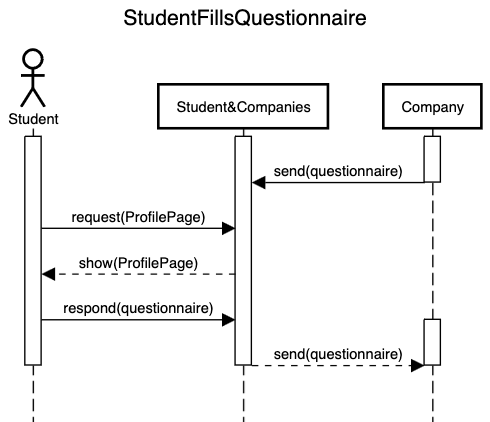
\includegraphics[width=0.8\textwidth]{../../assets/sequence-diagrams/StudentFillsQuestionnaire.png}
    }
\end{figure}

\item \subsubsection{CompanyAcceptsStudentEnrollment}

\begin{figure}[H]
    \centering
    \fcolorbox{black}{white}{
        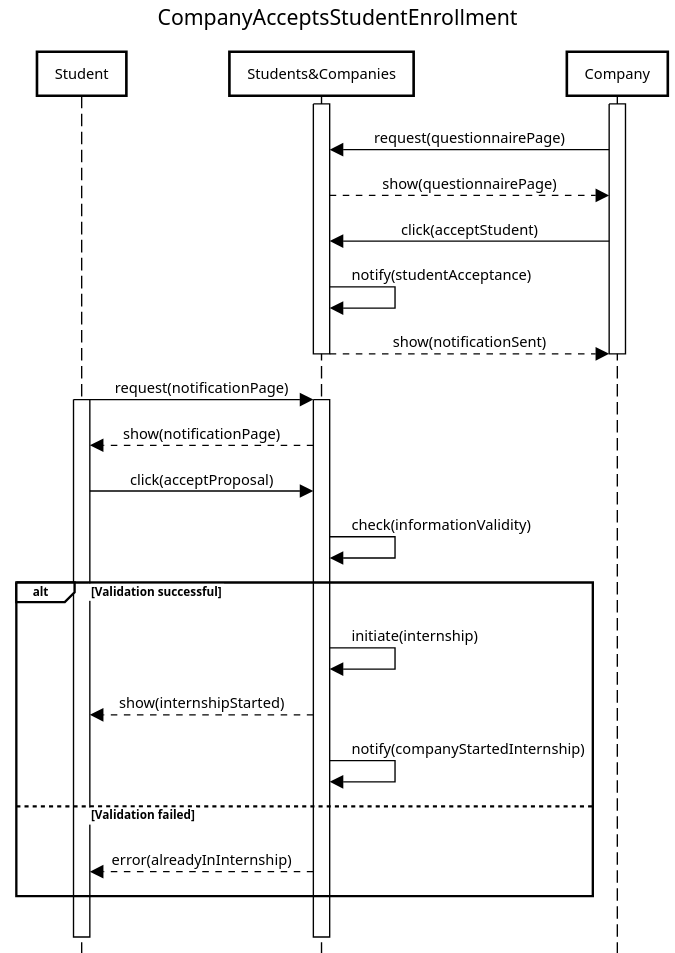
\includegraphics[width=0.8\textwidth]{../../assets/sequence-diagrams/CompanyAcceptsStudentEnrollment.png}
    }
\end{figure}

\item \subsubsection{StudentVisualizesInternshipInformation}

\begin{figure}[H]
    \centering
    \fcolorbox{black}{white}{
        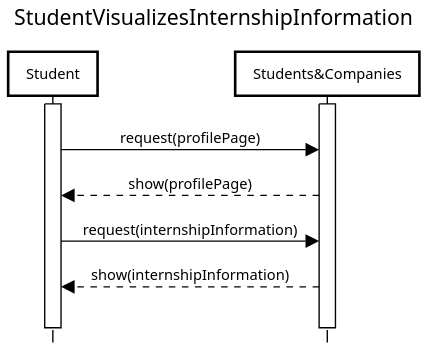
\includegraphics[width=0.5\textwidth]{../../assets/sequence-diagrams/StudentVisualizesInternshipInformation.png}
    }
\end{figure}

\item \subsubsection{CompanyVisualizesInternshipsInformation}

\begin{figure}[H]
    \centering
    \fcolorbox{black}{white}{
        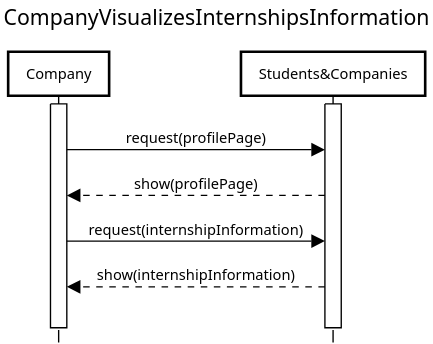
\includegraphics[width=0.5\textwidth]{../../assets/sequence-diagrams/CompanyVisualizesInternshipsInformation.png}
    }
\end{figure}

\item \subsubsection{StudentSendsComplaint}

\begin{figure}[H]
    \centering
    \fcolorbox{black}{white}{
        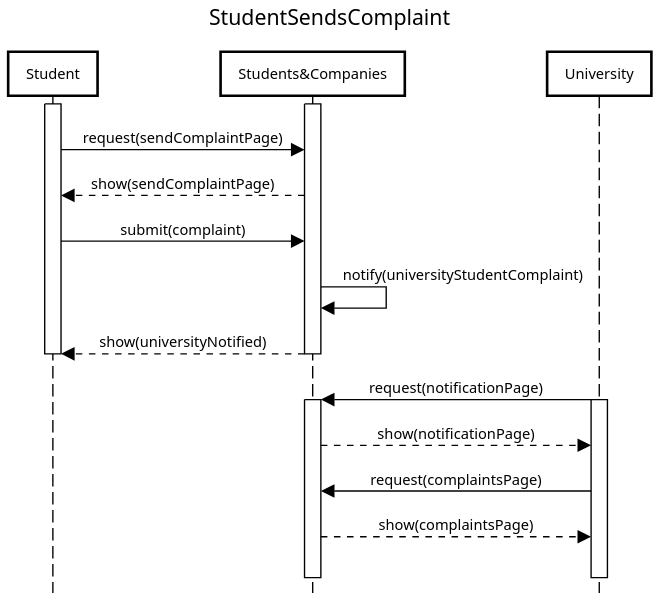
\includegraphics[width=0.8\textwidth]{../../assets/sequence-diagrams/StudentSendsComplaint.png}
    }
\end{figure}

\item \subsubsection{CompanySendsComplaint}

\begin{figure}[H]
    \centering
    \fcolorbox{black}{white}{
        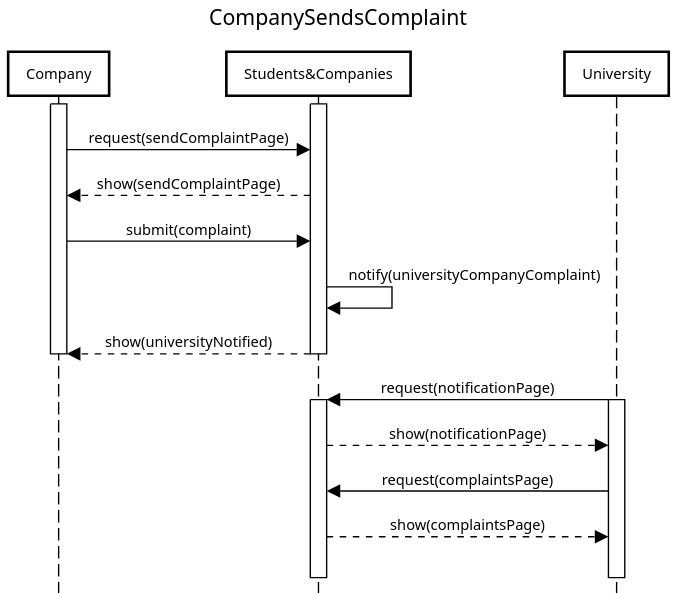
\includegraphics[width=0.8\textwidth]{../../assets/sequence-diagrams/CompanySendsComplaint.png}
    }
\end{figure}

\item \subsubsection{UniversityVisualizesComplaints}

\begin{figure}[H]
    \centering
    \fcolorbox{black}{white}{
        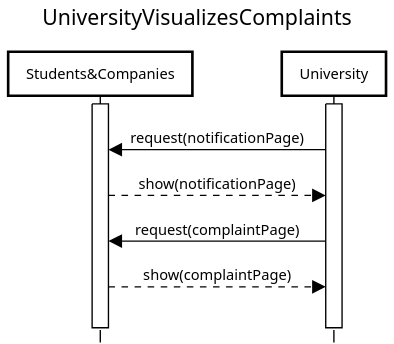
\includegraphics[width=0.5\textwidth]{../../assets/sequence-diagrams/UniversityVisualizesComplaints.png}
    }
\end{figure}

\item \subsubsection{UniversityEndsInternship}

\begin{figure}[H]
    \centering
    \fcolorbox{black}{white}{
        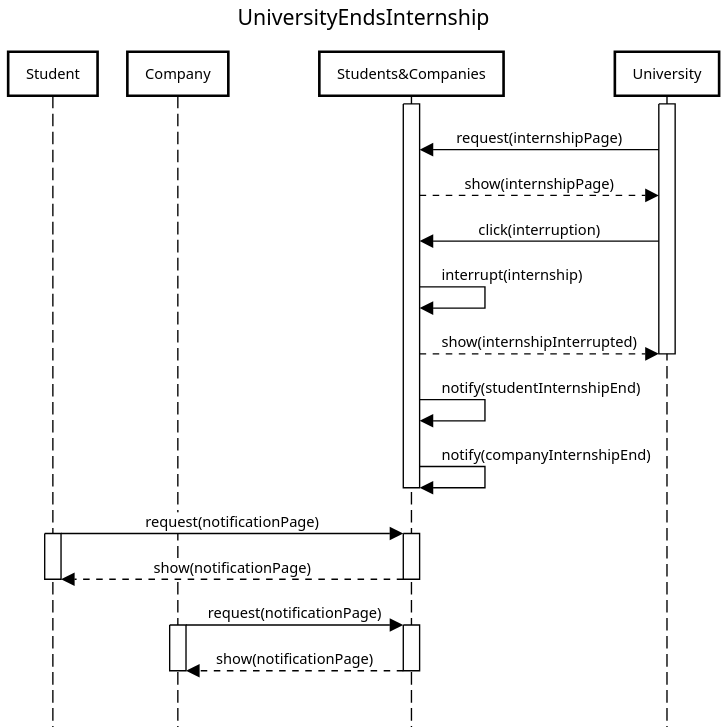
\includegraphics[width=0.8\textwidth]{../../assets/sequence-diagrams/UniversityEndsInternship.png}
    }
\end{figure}

\item \subsubsection{InternshipExpires}

\begin{figure}[H]
    \centering
    \fcolorbox{black}{white}{
        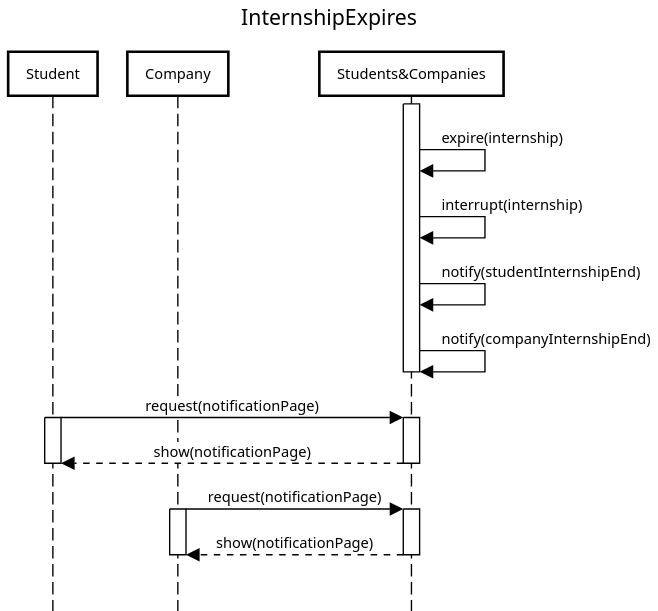
\includegraphics[width=0.8\textwidth]{../../assets/sequence-diagrams/InternshipExpires.png}
    }
\end{figure}

\item \subsubsection{StudentFillsFeedbackForm}

\begin{figure}[H]
    \centering
    \fcolorbox{black}{white}{
        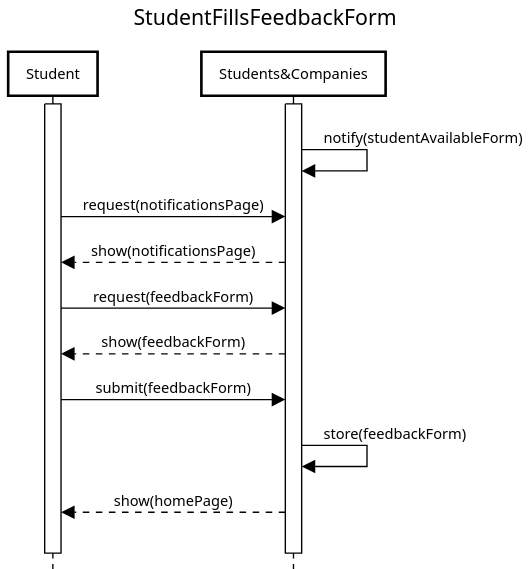
\includegraphics[width=0.5\textwidth]{../../assets/sequence-diagrams/StudentFillsFeedbackForm.png}
    }
\end{figure}

\end{enumerate}

\subsection{Use cases mapping}

\section{Performance requirements}

\subsection{Specific requirements}

\section{Design constraints}
\subsection{Standards compliance}
\subsection{Hardware limitations}
\subsection{Any other constraint}

\section{Software system attributes}
\subsection{Reliability}
\subsection{Availability}
\subsection{Security}
\subsection{Maintainability}
\subsection{Portability}